\section{太赫兹成像与传感领域}

第一幅太赫兹图像是由Hartwick等使用光学泵浦
的分子太赫兹激光器得到的。1995年,Hu和Nuss利
用基于飞秒激光源的光电太赫兹成像技术,在太赫兹科学
和技术领域引发了一波研究兴趣和活动。在过去的20年
里,太赫兹成像科学技术在基础研究和实际应用方面都取
得了巨大的进展。

\subsection{脉冲时域成像系统}

脉冲太赫兹TDS的核心技术使用飞秒激光器相干地产生和检测短脉冲。分束器(BS)用于将飞秒脉冲激光的近红外(NIR)光分成两部分:泵浦光束和探测光束。泵浦光束聚焦到一个有偏压的光电导天线表面,用于产生太赫兹。在外加电场下,飞秒激光脉冲在砷化镓晶体中产生的载流子产生瞬时电流,从而产生太赫兹频率的脉冲波。辐射的太赫兹脉冲被收集、准直,然后聚焦到被测样品上\cite{8702204}。

然后,从样品上反射回来的太赫兹脉冲被接收并聚焦到一个无偏压的光电导天线上,用于激光门控太赫兹检测。通常在太赫兹发射/接收天线上连接硅透镜(SL),可以提高太赫兹辐射耦合效率。通过用一个可变延迟电动平台来扫描近红外探测光束,以检测太赫兹脉冲的时间分辨电场。

\subsection{医疗和生物应用}

太赫兹辐射具有较低的光子能量(即非电离辐射),不会对人体造成任何安全风险。然而,它会因受到水的影响而强烈衰减,因此,太赫兹辐射对水含量非常敏感。在过去的10年里,人们对太赫兹光谱和成像在生物和医疗方面的应用越来越感兴趣。

2018年,Jung等使用太赫兹技术对早期宫颈癌患者淋巴结进行检测,实验对在体癌症引流区域的淋巴结进行分析成像,与术后淋巴结病理检查结果进行比较,结果发现淋巴结转移区域的反射峰振幅与正常淋巴结区域的反射峰振幅相比明显降低,太赫兹光谱成像能够显示最小约3 mm转移灶的轮廓。皮瓣是从人体健康处取下,带有血液供应的组织,其能否存活于损伤部位是皮瓣移植手术成功与否的关键。Bajwa及其同事将6只小鼠背部取得的皮瓣分成2组:皮瓣存活组和皮瓣坏死组(由组织学证实),使用太赫兹成像技术动态监测了一周内两组皮瓣含水量的变化,结果表明,太赫兹成像可以先于肉眼观察24h发现两组皮瓣的变化。Bajwa等的另一项研究同样是基于水含量的变化来探讨太赫兹成像对比(magnetic resonance imaging,MRI),从而来评估烧伤程度,这是首次体内评估太赫兹成像的水含量对比度和探测深度。此外,Hernandez-Cardoso及其同事将太赫兹成像技术在糖尿病的早期诊断中进行了测试。其中糖尿病组12人、对照组21人。受试者坐在特定的装置上,对足底进行太赫兹成像,分别比较了大拇趾、足底中部和脚后跟的数据后,结果均显示糖尿病组皮肤组织中水含量明显少于对照组,如图3所示。

\begin{figure}[htbp]
	\centering
	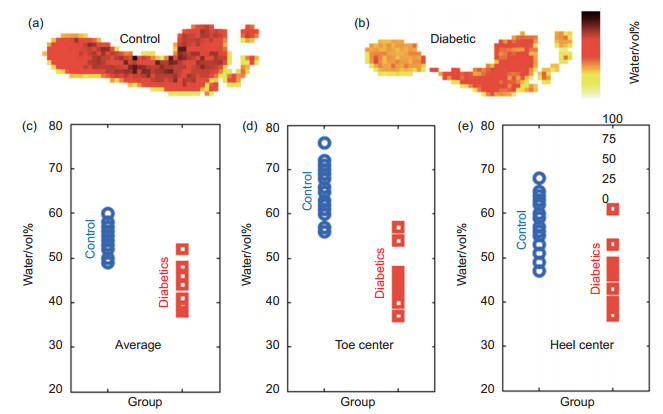
\includegraphics[width=0.6\textwidth]{img/img4.jpg} % 图片文件名,不需要加扩展名
	\caption{糖尿病足组与对照组的水含量的比较。(a)对照组太赫兹成像图;(b)糖尿病足组太赫兹成像图;(c)足底水含量;(d)拇趾中心水含量;(e)脚后跟中心水含量\cite{hernandez2017terahertz}}
	\label{fig:example}
\end{figure}